\usetikzlibrary{shapes.geometric}
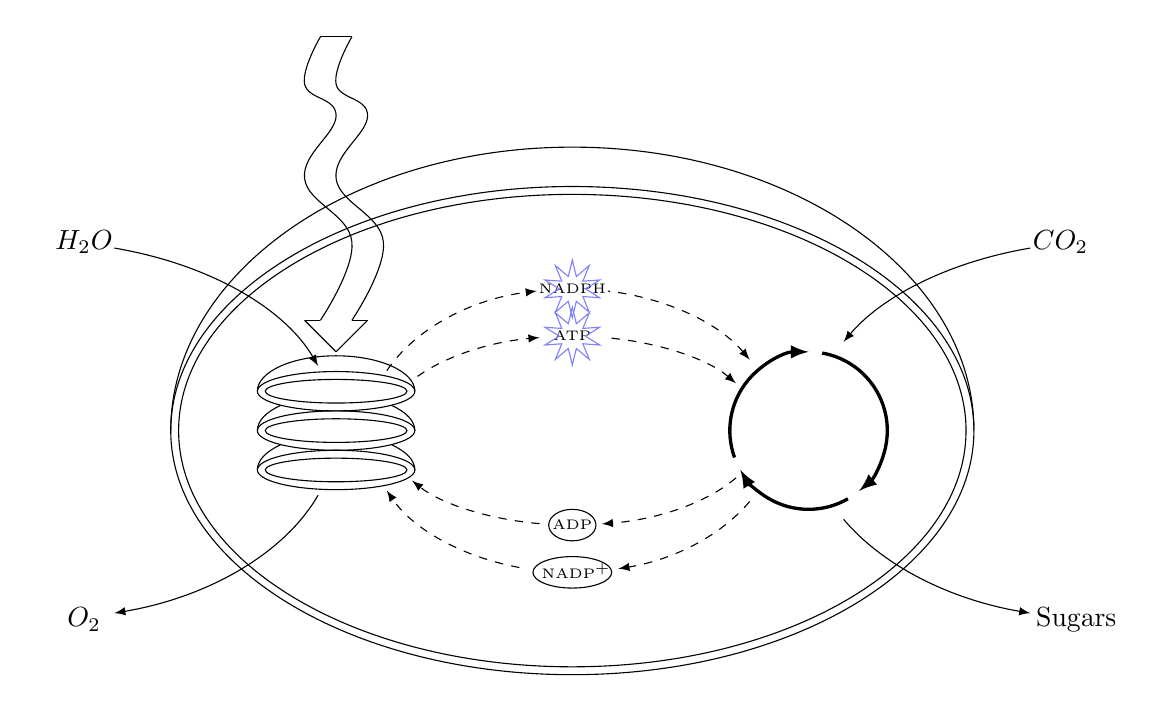
\begin{tikzpicture}
\node (center) at (0,0) {};
\draw  (center.center) ellipse (5 and 3); % cell membrane
\draw (center.center) ellipse (5.1 and 3.1); %cell membrane
\draw (center.center) +(0:5.1 and 3.6)arc(0:180:5.1 and 3.6);

\node (right) at (3,0) {};
\node (left) at (-3,0) {};
\node (l1) at (-3,0.5) {};
\node (l3) at (-3,-0.5) {};
% \draw (right.center) ellipse (1);


% Circular Arrows
\draw [very thick, - latex](3.1736,0.9848) arc (80.0026:-50:1);
\draw [very thick, - latex] (3.5,-0.866) arc (-59.9993:-150:1);
\draw [very thick, - latex] (2.0603,-0.342) arc (-160.0012:-270:1);

\node (rightE) at (6.8,0) {};
% \draw  (rightE) ellipse (3.8 and 2.4); % right reference ellipse
\draw [-latex] (rightE) +(105:3.8 and 2.4) arc(105:152:3.8 and 2.4);
\draw [latex-] (rightE) +(-105:3.8 and 2.4) arc(-105:-152:3.8 and 2.4);
\node at (6.2,2.4) {$CO_2$};
\node at (6.4,-2.4) {Sugars};
\node (leftE) at (-6.8,0) {};
% \draw  (leftE) ellipse (3.8 and 2.4); % left reference ellipse
\node at (-6.2,-2.4) {$O_2$};
\node at (-6.2,2.4) {$H_2O$};
\draw [-latex] (leftE)  +(75:3.8 and 2.4) arc(75:20:3.8 and 2.4);
\draw [latex-] (leftE)  +(-75:3.8 and 2.4) arc(-75:-20:3.8 and 2.4);

\draw  (left) ellipse (1 and .25); % middle thylakoid
\draw  (left) ellipse (.9 and .15); % middle thylakoid
\draw  (l1) ellipse (1 and .25); % top thylakoid
\draw  (l1) ellipse (.9 and .15); % top thylakoid
\draw  (l3) ellipse (1 and .25); %bottom thylakoid
\draw  (l3) ellipse (.9 and .15); % bottom thylakoid
\draw  (l1) +(0:1 and .45) arc(0:180:1 and .45);
\draw  (left) +(0:1 and .45) arc(0:45:1 and .45);
\draw  (left) +(180:1 and .45) arc(180:135:1 and .45);
\draw  (l3) +(0:1 and .45) arc(0:45:1 and .45);
\draw  (l3) +(180:1 and .45) arc(180:135:1 and .45);

% ATP / ADP Arrows
% \draw [dashed]  (center) ellipse (2.4 and 1.2); %reference ellipse
\draw [dashed,latex-]  (center) +(30:2.4 and 1.2) arc(30:80:2.4 and 1.2);
\draw [dashed,-latex]  (center) +(-30:2.4 and 1.2) arc(-30:-81:2.4 and 1.2);
\draw [dashed,-latex]  (center) +(-100:2.4 and 1.2) arc(-100:-148:2.4 and 1.2);
\draw [dashed,-latex]  (center) +(145:2.4 and 1.2) arc(145:100:2.4 and 1.2);

% NADPH / NADP^+ Arrows
\draw [dashed,latex-] (center) +(30:2.6 and 1.8) arc(30:80:2.6 and 1.8); 
\draw [dashed,-latex] (center) +(-30:2.6 and 1.8) arc(-30:-77:2.6 and 1.8);
\draw [dashed,-latex] (center) +(-105:2.6 and 1.8) arc(-105:-155:2.6 and 1.8);
\draw [dashed,-latex] (center) +(155:2.6 and 1.8) arc(155:100:2.6 and 1.8);

\node (B) at (0,1.2) {\tiny ATP};
\node[ % ATP Star
       star,
       star points=10,
       star point height=2mm,
       %ball color=violet,
       draw=blue!50,
       font=\bf
    ] at (B.center) {};
    
\node (C) at (0,1.8) {\tiny NADPH};    
\node[ % NADPH Star
       star,
       star points=10,
       star point height=2mm,
       %ball color=violet,
       draw=blue!50,
       font=\bf
    ] at (C.center) {};
    
\node (ADP) at (0,-1.2) {\tiny ADP};
\draw (ADP) ellipse (0.3 and 0.2); % ADP ellipse

\node (E) at (0,-1.8) {}; %NADP+ ellipse
\node at (0.05,-1.78) {\tiny NADP$^+$};
\draw  (E) ellipse (0.5 and 0.2); % NADP+ ellipse

%  Sun Arrow
\node (sun1) at (-3.2,5) {};
\node (sun2) at (-3.4,4.4) {};
\node (sun3) at (-3.0,4) {};
\node (sun4) at (-3.4,3.2) {};
\node (sun5) at (-2.8,2.4) {};
\node (sun6) at (-3.2,1.4) {};

\node (sun7) at (-2.8,5) {};
\node (sun8) at (-3.0,4.4) {};
\node (sun9) at (-2.6,4) {};
\node (sun10) at (-3.0,3.2) {};
\node (sun11) at (-2.4,2.4) {};
\node (sun12) at (-2.8,1.4) {};

\node (sunFinal) at (-3,1) {};
\draw plot[smooth, tension=.7] coordinates {(sun1) (sun2) (sun3) (sun4) (sun5) (sun6)};
\draw plot[smooth, tension=.7] coordinates {(sun7) (sun8) (sun9) (sun10) (sun11) (sun12)};

\node (sunR) at (-2.6,1.4) {};
\node (sunL) at (-3.4,1.4) {};
\draw (sun12.center) -- (sunR.center);
\draw (sunR.center) -- (sunFinal.center);
\draw (sun6.center) -- (sunL.center);
\draw (sunL.center) -- (sunFinal.center);
\draw (sun1.center) -- (sun7.center);

\node at (-3.2,1.4) {};
\end{tikzpicture}